\section{Experiments}
\label{sec:experiments}
In this section, we demonstrate our method's effectiveness. We first compare our results with the SoTA works using the ResNet architectures on CIFAR \cite{krizhevsky2009learning} and ImageNet-1k \cite{deng2009imagenet}, then
conduct ablation studies to verify different aspects of our method, including \textbf{(1)} each proposed technology's verification, \textbf{(2)} our method's extension to spiking self-attention \cite{zhou2022spikformer}, \textbf{(3)} conquering the “temporal constraint” of the prior arts \cite{shen2024conventional} on the event dataset CIFAR10-DVS \cite{li2017cifar10}, and \textbf{(4)} the learned bit allocation's visualization. \emph{All Implementation Details Are Attached in the Appendix.} 

\subsection{Comparisons with existing works}
\label{sbsec:comparison}
\textbf{CIFAR.} We apply our method to ResNet20 \cite{guo2024ternary} to compete with the SoTA SNNs. As shown in  \cref{tab:comparison on cifar}, we first compare our method with those learning- or module-based model optimization, \eg,  \cite{li2021differentiable, deng2021temporal, zheng2021going}, to prove our solution of non-differentiable terms performs well. Then, we compare with multi-bit SNNs, \eg,  \cite{guo2024ternary,xiao2024multi}, to prove we can achieve higher accuracy while using much lower memory (bit budget) and computation (S-ACE). Finally, compared with plain uniform quantization, our work can further squeeze the model accuracy to its limit while maintain lower memory and computation overhead, proving the effectiveness of adaptive bit allocation. Additionally, since we adopt the temporal squeezing technique as shown in  \cref{eq:our sn1} and  \cref{fig:overview}, the temporal dimension could also be compressed to 1 timestep before performing convolution, making sequential processing of SNNs more efficient during inference. That's why in the case of “W/S/T=222”, S-ACE can be further decreased. More elaborations on this are deferred to the appendix for better understanding.
\\\textbf{ImageNet.} We further apply our method to SEW-ResNet34 to demonstrate the superiority on the up-scaled dataset. As listed in  \cref{tab:comparison on imagenet}, compared with those using improved learning techniques or special modules  \cite{rathi2020enabling, zheng2021going,li2021differentiable,hu2024advancing}, we can achieve magnitudes of memory and computation savings without using any of their tricks. Furthermore, we can save 91.2\% memory (5.61 \vs64) and  85.83\% computation (30.74 \vs217) while achieve a higher accuracy (70.57\% \vs70.13\%) when compared with the quantized SNN. As bit budget increases, we can push accuracy to the advanced 72.82\% while still maintain lower memory and computation overhead, outperforming full-precision SNNs  \cite{guo2024ternary, fang2021deep, deng2021temporal}.

\subsection{Ablation study}
\label{sbsec:ablation}
We first continue to use ResNet20 and CIFAR10 to conduct ablation studies on the proposed techniques. Then, we migrate the proposed method to a different architecture Spikformer \cite{zhou2022spikformer} to further verify  effectiveness. On the extension to the event dataset, we push our method to conquer the “temporal constraint” issue, which doubles the prior art \cite{shen2024conventional}. 
Finally, we visualize the learned bit allocation. 
\\\textbf{Effectiveness of learnable bit width and the renew mechanism.} 
We first perform the plain uniform quantization (U-quant.) as the baselines, following  \cite{shen2024conventional}. As shown in \cref{exp:ablation on learnable bit}, the proposed learnable bit width technology (LBW) consistently outperforms U-quant, managing to allocate correct bit widths to different layers and improving the model accuracy to a higher level. Furthermore, we add the proposed renew mechanism only to the spike activation ($V_{th,l}^1$, Act.-only), or only to the weight ($S_q^l$, Weight-only), or to the bilateral case ($V_{th,l}^1$ and $S_q^l$). The results coherently show the renew mechanism can further improve LBW outcomes, mitigating the step-size mismatch issue.
As illustrated before, SNN would severely  suffer from the additional temporal quantization error. That's why Act.-only renew alone is effective enough to produce the best results. Bilateral renew seconds due to  a slightly lower bit budget. For simplicity, we adopt \emph{the 
Act.-only renew as the main method by default}.
\begin{table}[t]
\centering
\caption{Ablations on learnable bit width (LBW) and the renew mechanism. Different fonts denote the \textbf{1st}, the 
{\color[HTML]{9B9B9B} \textbf{2nd}}, and the  {\ul 3rd} best results, respectively. LBW models are initial to W/S/T=4/4/2.}
\label{exp:ablation on learnable bit}
\begin{adjustbox}{max width=0.49\textwidth}
\begin{threeparttable}
\begin{tabular}{c|c|cc||cc|cc|cc}
\toprule
\textbf{Target}         & \textbf{U-quant.} & \multicolumn{2}{c||}{\textbf{LBW}} & \multicolumn{2}{c|}{\textbf{\begin{tabular}[c]{@{}c@{}}LBW\\ +Weight-only Renew\end{tabular}}} & \multicolumn{2}{c|}{\textbf{\begin{tabular}[c]{@{}c@{}}LBW\\ +Bilateral Renew\end{tabular}}} & \multicolumn{2}{c}{\textbf{\begin{tabular}[c]{@{}c@{}}LBW\\ +Act.-only Renew\end{tabular}}} \\ \midrule
\textbf{W/S/T} & \textbf{Top-1}    & \textbf{W/S/T}  & \textbf{Top-1}  & \textbf{W/S/T}                                 & \textbf{Top-1}                                & \textbf{W/S/T}                    & \textbf{Top-1}                                           & \textbf{W/S/T}                    & \textbf{Top-1}                                          \\ \midrule
1/1/1          & 74.82             & 1.60/1.91/1.0   & {\ul 95.65}     & 1.73/1.98/1.0                                  & 93.28                                         & 1.25/1.36/1.0                     & {\color[HTML]{9B9B9B} \textbf{95.84}}                    & 1.38/1.32/1.0                     & {\color[HTML]{000000} \textbf{96.15}}                   \\
1/2/1          & 86.8              & 1.48/2.00/1.0   & {\ul 95.55}     & 1.57/2.12/1.0                                  & 93.52                                         & 1.25/2.04/1.0                     & {\color[HTML]{9B9B9B} \textbf{96.25}}                    & 1.42/2.08/1.0                     & \textbf{96.58}                                          \\
2/2/1          & 88.65             & 1.88/2.06/1.0   & 94.62           & 1.99/2.06/1.0                                  & {\ul 95.71}                                   & 2.00/1.89/1.0                     & {\color[HTML]{9B9B9B} \textbf{96.47}}                    & 2.08/2.08/1.0                     & \textbf{96.51}                                          \\
2/3/1          & 93.64             & 2.10/3.00/1.0   & 96.37           & 1.96/3.00/1.0                                  & {\ul 96.51}                                   & 2.02/3.06/1.0                     & {  \textbf{96.97}}                    & 2.24/3.06/1.0                     & {\color[HTML]{9B9B9B} \textbf{96.63}}                   \\
3/3/1          & 95.38             & 3.01/2.95/1.0   & 96.34           & 3.00/3.06/1.0                                  & {\ul 96.66}                                   & 2.87/3.04/1.0                     & {\color[HTML]{9B9B9B} \textbf{96.77}}                    & 2.89/2.87/1.0                     & \textbf{96.90}                                          \\
3/4/1          & 96.09             & 2.87/4.10/1.0   & 96.72           & 2.90/3.98/1.0                                  & {\ul 96.89}                                   & 2.97/3.94/1.0                     & {\color[HTML]{9B9B9B} \textbf{97.01}}                    & 3.01/4.00/1.0                     & \textbf{97.02}                                          \\
4/4/1          & 96.35             & 4.04/4.06/1.0   & 96.78           & 3.99/4.02/1.0                                  & {\ul 97.00}                                   & 3.86/4.00/1.0                     & {\color[HTML]{9B9B9B} \textbf{97.03}}                    & 3.99/4.06/1.0                     & \textbf{97.05}                                          \\
4/4/2          & 96.39             & 4.02/3.93/1.92  & {\ul 96.80}     & 3.88/4.04/2.0                                  & 96.57                                         & 4.01/3.97/2.0                     & {  \textbf{97.03}}                    & 3.93/4.03/2.08                    & {\color[HTML]{9B9B9B} \textbf{96.92}}                   \\ \bottomrule
\end{tabular}
% \begin{tablenotes}
% \footnotesize
% \item $\dagger$ denotes plain uniform quantization, following  \cite{shen2024conventional}.
% \item $*$ denotes the temporal squeezing is applied in inference.
% \end{tablenotes}
\end{threeparttable}
\end{adjustbox}
\end{table}
\begin{table}[t]
\centering
\caption{Ablations on the refined spiking neuron. Different fonts denote the \textbf{1st}, the 
{\color[HTML]{9B9B9B} \textbf{2nd}}, and the  {\ul 3rd} best results, respectively.}
\label{exp:ablation on refined neuron}
\begin{adjustbox}{max width=0.48\textwidth}
\begin{threeparttable}
\begin{tabular}{c|c|cc|cc|cc|cc}
\toprule
{  \textbf{Target} }                                                                                  & {  \textbf{\begin{tabular}[c]{@{}c@{}}$\tau=2$\& \cref{eq:mlif3} \\ U-quant.\end{tabular}}} & \multicolumn{2}{c|}{{  \textbf{\begin{tabular}[c]{@{}c@{}}$\tau=2$\& \cref{eq:mlif3}  \\ w/o renew\end{tabular}}}} & \multicolumn{2}{c|}{{  \textbf{\begin{tabular}[c]{@{}c@{}}$\tau=2$\& \cref{eq:mlif3} \\ w/ renew\end{tabular}}}} & \multicolumn{2}{c|}{{  \textbf{\begin{tabular}[c]{@{}c@{}}$\tau=2$\& \cref{eq:our sn3}\\ w/ renew\end{tabular}}}} & \multicolumn{2}{c}{{  \textbf{\begin{tabular}[c]{@{}c@{}}$\tau=1$\& \cref{eq:our sn3}\\ w/ renew\end{tabular}}}} \\ \midrule
{  \textbf{ W/S/T}} & {  \textbf{Top-1}}                                                       & {  \textbf{W/S/T}}                    & {  \textbf{Top-1}}                   & {  \textbf{W/S/T}}                   & {  \textbf{Top-1}}                  & {  \textbf{W/S/T}}                   & {  \textbf{Top-1}}                  & {  \textbf{W/S/T}}                  & {  \textbf{Top-1}}                  \\ \midrule
{  1/1/1}                                                                              & {  74.82}                                                                & {  1.80/2.14/1.0}                     & {  95.12}                            & {  1.80/2.09/1.0}                    & {  {\ul 95.58}}                     & {  1.46/1.34/1.0}                    & {\color[HTML]{9B9B9B} \textbf{95.71}}                  & {  1.38/1.32/1.0}                   & {  \textbf{96.15}}                  \\
{  1/2/1}                                                                              & {  10.02}                                                                & {  1.77/2.2/1.0}                      & {  95.21}                            & {  1.58/2.13/1.0}                    & {  {\ul 96.14}}                     & {  1.40/2.05/1.0}                    & {\color[HTML]{9B9B9B} \textbf{96.48}}                  & {  1.42/2.08/1.0}                   & {  \textbf{96.58}}                  \\
{  2/2/1}                                                                              & {  0.1}                                                                  & {  2.10/2.07/1.0}                     & {  95.50}                            & {  2.09/1.97/1.0}                    & {  {\ul 96.04}}                     & {  1.88/1.95/1.0}                    & {\color[HTML]{9B9B9B} \textbf{96.45}}                  & {  2.08/2.08/1.0}                   & {  \textbf{96.51}}                  \\
{  2/3/1}                                                                              & {  89.06}                                                                & {  2.05/3.01/1.0}                     & {  {\ul 96.51}}                      & {  2.13/3.16/1.0}                    & {  96.38}                           & {  1.96/3.04/1.0}                    & {  \textbf{96.72}}                  & {  2.24/3.06/1.0}                   & {\color[HTML]{9B9B9B} \textbf{96.63}}                  \\
{  3/3/1}                                                                              & {  0.1}                                                                  & {  2.98/3.02/1.0}                     & {  96.18}                            & {  3.01/3.07/1.0}                    & {  {\ul 96.43}}                     & {  3.03/3.01/1.0}                    & {\color[HTML]{9B9B9B} \textbf{96.82}}                  & {  2.89/2.87/1.0}                   & {  \textbf{96.90}}                  \\
{  3/4/1}                                                                              & {  96.31}                                                                & {  3.06/3.98/1.0}                     & {  96.64}                            & {  2.99/4.02/1.0}                    & {  {\ul 96.80}}                     & {  2.95/4.06/1.0}                    & {\color[HTML]{9B9B9B} \textbf{97.00}}                  & {  3.01/4.0/1.0}                    & {  \textbf{97.02}}                  \\ \bottomrule
\end{tabular}
% \begin{tablenotes}
% \footnotesize
% \item $\dagger$ denotes plain uniform quantization, following  \cite{shen2024conventional}.
% \item $*$ denotes the temporal squeezing is applied in inference.
% \end{tablenotes}
\end{threeparttable}
\end{adjustbox}
\end{table}
\begin{table}[b]
\centering
\caption{Ablations of Spikformer-4-384 on CIFAR10. Different fonts denote the \textbf{1st} and the 
{\color[HTML]{9B9B9B} \textbf{2nd}} best results, respectively.}
\label{exp:ablation of spf}
\begin{adjustbox}{max width=0.46\textwidth}
\begin{threeparttable}
\begin{tabular}{c|c|cc|cc|cc}
\toprule
{ \textbf{ Target }}                                                                                   & {  \textbf{U-quant.}} & \multicolumn{2}{c|}{{  \textbf{LBW}}}                & \multicolumn{2}{c|}{{  \textbf{LBW + renew}}}                 & \multicolumn{2}{c}{\textbf{Origin \cite{zhou2022spikformer}}}          \\ \midrule
{  \textbf{W/S/T}} & {  \textbf{Top-1}}    & {  \textbf{W/S/T}} & {  \textbf{Top-1}} & {  \textbf{W/S/T}} & {  \textbf{Top-1}} & \textbf{W/S/T}           & Top-1                   \\ \midrule
{  1/1/1}                                                                              & {  79.53}             & {  1.44/1.48/1.0}  & {\color[HTML]{9B9B9B} \textbf{95.37}} & {  1.53/1.5/1.0}   & {  \textbf{95.47}} &                          &                         \\
{  1/2/1}                                                                              & {  89.3}              & {  1.47/1.99/1.0}  & {  \textbf{95.68}} & {  1.47/2.01/1.0}  & {\color[HTML]{9B9B9B} \textbf{95.54}} &                          &                         \\
{  2/2/1}                                                                              & {  89.68}             & {  1.88/2.03/1.0}  & {\color[HTML]{9B9B9B} \textbf{95.80}} & {  2.02/2.01/1.0}  & {  \textbf{95.84}} &                          &                         \\
{  2/3/1}                                                                              & {  94.11}             & {  2.00/2.94/1.0}  & {\color[HTML]{9B9B9B} \textbf{95.93}} & {  2.15/2.95/1.0}  & {  \textbf{96.04}} &                          &                         \\
{  3/3/1}                                                                              & {  94.21}             & {  2.93/3.01/1.0}  & {\color[HTML]{9B9B9B} \textbf{95.87}} & {  2.89/2.99/1.0}  & {  \textbf{95.99}} & \multirow{-5}{*}{16/1/4} & \multirow{-5}{*}{95.19} \\ \bottomrule
\end{tabular}

% \begin{tablenotes}
% \footnotesize
% \item $\dagger$ denotes plain uniform quantization, following  \cite{shen2024conventional}.
% \item $*$ denotes the temporal squeezing is applied in inference.
% \end{tablenotes}
\end{threeparttable}
\end{adjustbox}
\end{table}
\\\textbf{Importance of the refined spiking neuron.}
We further verify the effectiveness of the refined spiking neuron. The major differences are that we refine  \cref{eq:mlif3} to  \cref{eq:our sn3} and suggest using the IF neuron rather than LIF, \ie, using $\tau=1$ rather than the default $\tau=2$ \cite{fang2023spikingjelly}. In  \cref{exp:ablation on refined neuron}, the results consistently show that the original multi-bit neuron would impair the quantized model's robustness, while our refining tricks and renew mechanism steadily improve the model performance to better states. Thus, enabling the advancement of high-performance and low-overhead SNNs. 
\begin{table}[t]
\centering
\caption{Spikformers on CIFAR10-DVS. The \textbf{best results} and {\ul temporal lengths} are highlighted.}
\label{exp:ablations on dvs}
\begin{adjustbox}{max width=0.45\textwidth}
\begin{threeparttable}
\begin{tabular}{cc|cc|cc}
\hline
\multicolumn{2}{c|}{\textbf{Origin} \cite{shen2024conventional}}             & \multicolumn{2}{c|}{\textbf{Quant. Spkiformer} \cite{shen2024conventional}} & \multicolumn{2}{c}{\textbf{Our Spkiformer}} \\ \hline
\textbf{W/S/T}           & \textbf{Top-1}        & \textbf{W/S/T}      & \textbf{Top-1}      & \textbf{W/S/T}    & \textbf{Top-1}    \\ \hline
\multirow{5}{*}{16/1/16} & \multirow{5}{*}{80.7} & 1/1/{\ul16}             & \textbf{79.8}       & 1.11/2.00/{\ul6.0}     & \textbf{80.9}     \\
                         &                       & 1/2/{\ul8}             & 79.3                & 1.28/2.00/{\ul4.0}     & 80.0              \\
                         &                       & 1/4/{\ul4}            & 63.1                & 1.33/4.00/{\ul3.0}     & 80.1              \\
                         &                       & 1/8/{\ul2}            & 43.0                & 1.31/4.03/{\ul2.0}     & 78.7              \\
                         &                       & 1/16/{\ul1}          & 35.8                & 1.31/4.03/{\ul1.0}     & 77.4              \\ \hline
\end{tabular}
% \begin{tablenotes}
% \footnotesize
% \item \textbf{TS} abbreviates temporal squeezing.
% \end{tablenotes}
\end{threeparttable}
\end{adjustbox}
\end{table}
\begin{figure}[b]
  \centering
  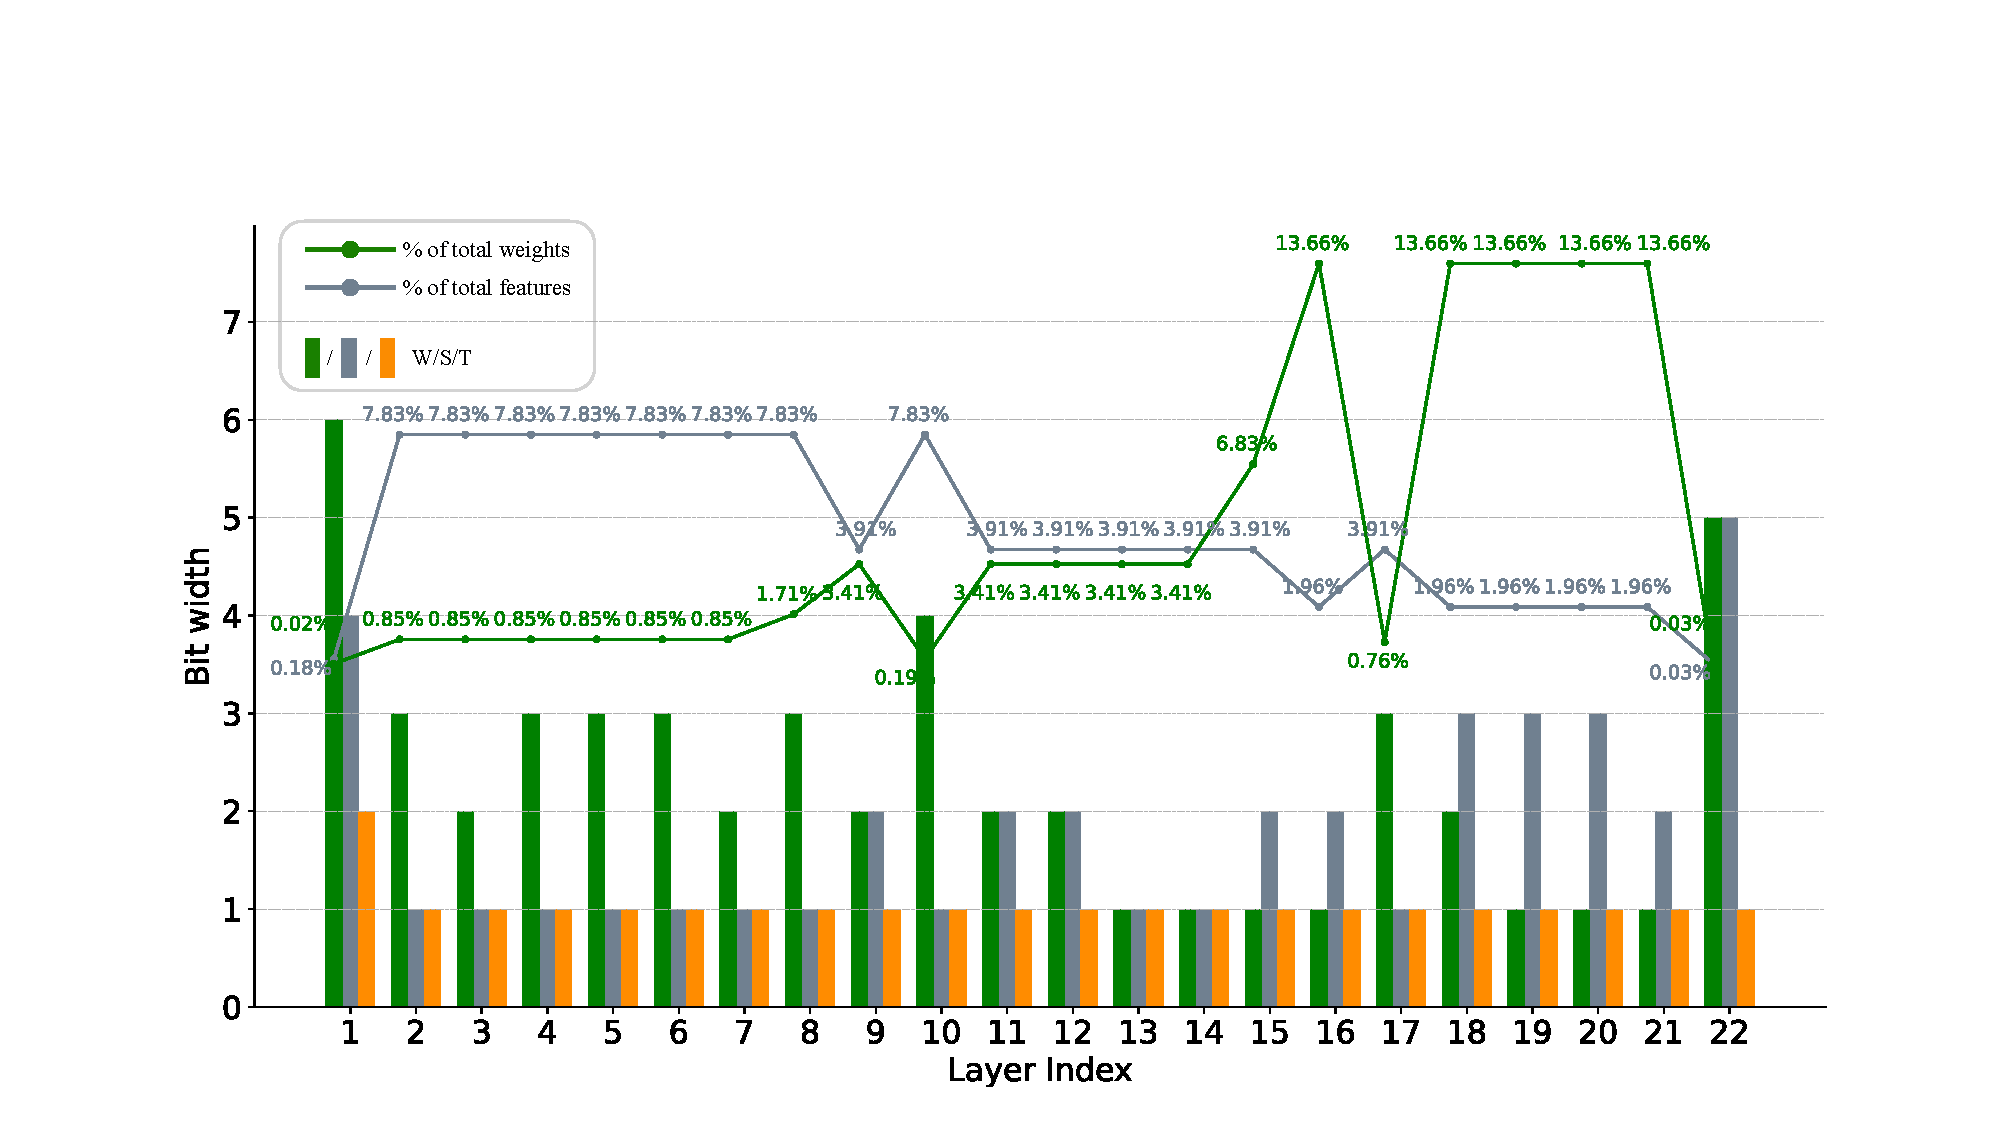
\includegraphics[width= 8cm]{figs/bit_vis.pdf}
  \caption{Statistics of each layer's bit widths. Since layer \#1 has two time-steps, we report the averaged spike bit width for clarity.}
  \label{fig:bit_vis}
\end{figure}
\\\textbf{Validation on spiking self-attention architectures.}
We then consider a new architecture Spikformer. Migrating our method to Spikformer is \textbf{non-trivial} because the self-attention operation is a different computing paradigm where a new quantizable tensor $atten$ arises. We would like to leave room for future work. Here, we naively apply our method to Spikformer as depicted in  \cref{fig:intro} to validate migratability.  We adopt the default Spikformer-4-384 \cite{zhou2022spikformer} on CIFAR10. As listed in  \cref{exp:ablation of spf}, with our LBW, the model accuracy surpasses the original Spikformer under the same hyperparameters, while plain quantization fails. Adding the the renew mechanism would further boost the performance.
\\\textbf{Conquering the temporal constraint.}
We further test the migratability on the special event dataset. We use the same default Spikformer and settings as  \cite{shen2024conventional} without any data augmentation. As shown in  \cref{exp:ablations on dvs}, “temporal constraint” refers to the dramatic accuracy decrease of event datasets as temporal length declines to the extremely low time-step \cite{shen2024conventional}. However, in our work, such phenomenon disappears and accuracy is well maintained even in the case of $T=1$. 
This implies that spatial information can be better extracted with our method even in the sparse event data.
Meanwhile, we are in line with prior findings that temporal information matters more than spatial information to event datasets. 
Moreover, compared with the original Spkiformer, our method can achieve higher accuracy with lower bit budgets
and time steps, proving the effectiveness on event data.
\\\textbf{Statistics of bit widths.} Last but not least, we visualize the learned bit allocation of ResNet20 with W/S/T = 1.38/1.32/1 on CIFAR10 to visually confirm effectiveness. Notably, different from any prior arts \cite{guo2024ternary,zheng2021going,fang2021deep}, we add additional spiking neurons before the first layer to fully benefit the model with addition-only computation. In consistence with the previous setting, the model is initialized to W/S/T = 4/4/2. 
As vividly displayed in  \cref{fig:bit_vis}, \textbf{(1)} the layers with the higher proportion of feature and weight tend to get lower bits thus lowering the overall memory and computation. \textbf{(2)} The 1st and last layers tend to learn higher bit widths, which is line with their outstanding importance as reported in prior arts \cite{choi2018pact}. With \textbf{(1)} and \textbf{(2)} combined, we conclude our adaptive bit allocation method should be sensible and effective.







% \begin{table}[t]
% \centering
% \caption{Comparisons with existing works on ImageNet.}
% \label{exp:comparison with ann baseline}
% \begin{adjustbox}{max width=0.48\textwidth}
% \begin{threeparttable}

% % \begin{tablenotes}
% % \footnotesize
% % \item $\dagger$ denotes plain uniform quantization, following  \cite{shen2024conventional}.
% % \item $*$ denotes the temporal squeezing is applied in inference.
% % \end{tablenotes}
% \end{threeparttable}
% \end{adjustbox}
% \end{table}

\section{Conclusion}
\label{sec:conclusion}
In this paper, we propose an adaptive bit allocation method, based on learnable bit widths, for efficient and accurate SNNs. 
To solve the new challenges brought by the special temporal dimension of SNN, we refine the spiking neuron to enable temporal matching inter- and intra-layer and increase the adaptivity via better neuron formulations for better model performance. We further theoretically formulate the step size mismatch issue that would temporally deteriorate, and alleviate it by the proposed renew mechanism.
Thorough experiments are conducted to prove every aspects is effective. 
Eventually, we advance accuracy with lower memory (Bit budget) and computation (S-ACE) overhead.